\documentclass{beamer}

\usepackage[utf8]{inputenc}
\usetheme{Madrid}
\usepackage{amssymb}
\usepackage{enumitem}
\usepackage{graphicx}
\graphicspath{ {./images/} }
\setitemize{label=\usebeamerfont*{itemize item}%
	\usebeamercolor[fg]{itemize item}
	\usebeamertemplate{itemize item}}

%Information to be included in the title page:
\title[Introductory Talk] %optional
{Overfitting and Generalization Performance}





\begin{document}
	
\frame{\titlepage}
	
\begin{frame}
\frametitle{Introduction}
	
	\begin{block}{General Aim}
		Given training sample \[(x_1, y_1), ..., (x_n, y_n) \in \mathbb{R}^d \times \mathbb{R}\]
		learn a predictor 
		$h_n : \mathbb{R}^d \to \mathbb{R}$ that predicts $y$ given new $x$.
	\end{block}
	
	\begin{block}{Empirical Risk Minimization (ERM)}
		Minimize training risk:
		$\frac{1}{n} \sum_{i=1}^{n}\ell(h(x_i), y_i) $
		given a loss function $\ell$.
	\end{block}

\end{frame}

\begin{frame}
\frametitle{Generalization}

\begin{itemize}[itemsep = 12pt]
	\item Find $h_n$ that performs well on unseen data.
	\item Minimize true risk: $E[\ell (h(x), y)]$
where  $(x, y)$ drawn independently from $P$.
\end{itemize}

\end{frame}

\begin{frame}
\frametitle{"Classical" thinking}
\begin{itemize}[itemsep = 12pt]
	\item Finding a balance between underfitting and overfitting.
	\item "Bias-Variance Tradeoff"
	\item 0 training error does not tend to generalize well.
	\item Control function class $\mathcal{H}$ implicitly or explicitly.
\end{itemize}
\end{frame}


\begin{frame}
\frametitle{Generalization of performance}
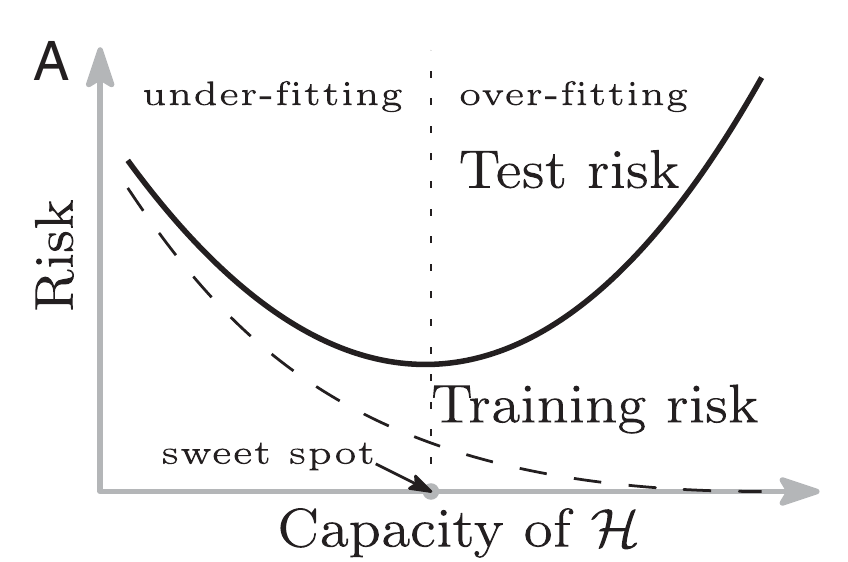
\includegraphics[height=6cm]{UCurve.png}
\\Classical curve from bias variance tradeoff.
\end{frame}

\begin{frame}
\frametitle{Modern practice}
\begin{itemize}[itemsep = 12pt]
	\item Modern ML methods such as large neural networks and other non-linear predictors have very low to no training risk
	\item NN architectures chosen such that interpolation can be achieved.
	\item Works even when training data have high levels of noise.
\end{itemize}
\end{frame}

\begin{frame}
\frametitle{"Double Descent"}
\begin{itemize}[itemsep = 12pt]
	\item "Double Descent" curve proposed and empirically observed to some extent.
	\item Curve the extends beyond the point of interpolation
	\item Risk decreases beyond this point, typically surpassing performance of classical stopping point.
\end{itemize}
\end{frame}

\begin{frame}
\frametitle{Double Descent Curve}
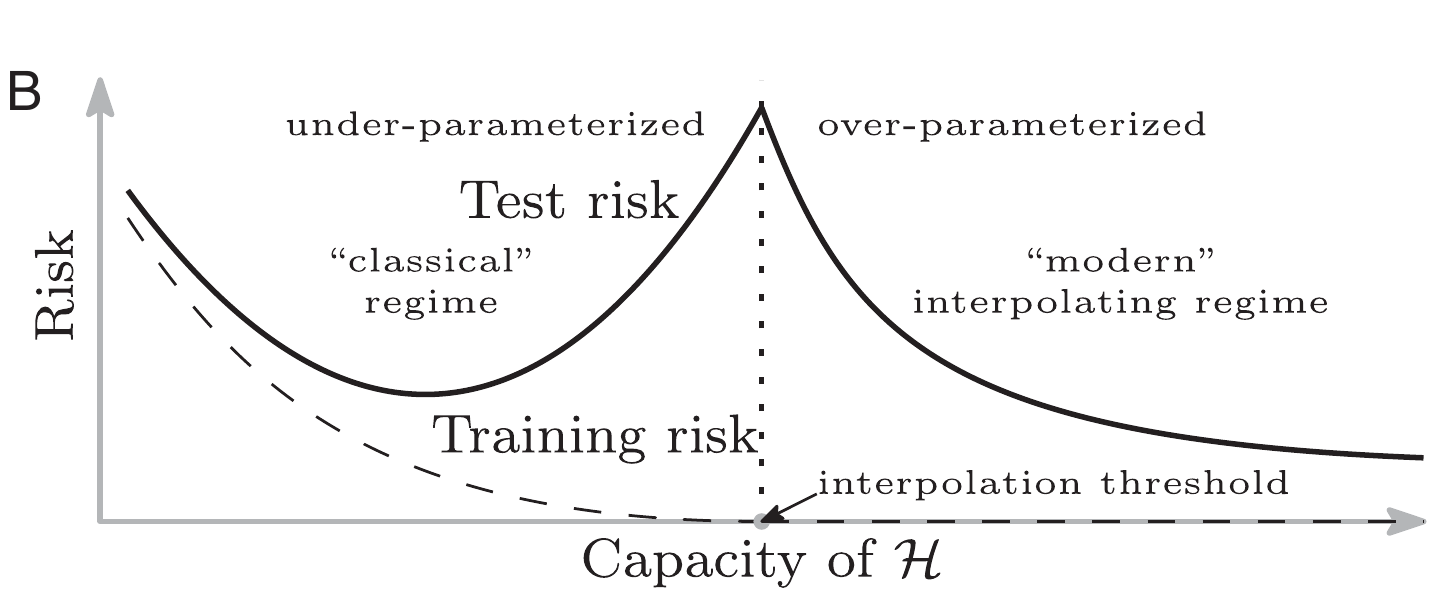
\includegraphics[height=5cm]{Double-Descent-Curve.png}
\end{frame}

\begin{frame}
\frametitle{Explanations on Double Descent}
Why should the test risk decrease even when empirical risk stays the same?\\
\begin{itemize}[itemsep = 12pt]
	\item Capacity of function class needs not suit the appropriate inductive bias for the problem.
	\item By having a larger function class, may find a function that matches the inductive bias better.
	\item Eg., smoother function, smaller norm, larger margin.
\end{itemize}

\end{frame}

\begin{frame}
\frametitle{Empirical Evidence - Random Fourier Features}
Let the function class  $\mathcal{H}_\infty$ be the Reproducing Kernel Hilbert Space (RKHS) corresponding to the Gaussian kernel.\\
We consider the following non-linear parametric model:
\begin{block}{Random Fourier Features (RFF)}
	Let the function class  $\mathcal{H}_N $ consist of functions $h_n : \mathbb{R}^d \to \mathbb{C}$ of the form:
	\[ h(\cdot) = \sum_{k=1}^{N} a_k\phi(\cdot, v_k) \] 
	where $\phi(\cdot , v_k) := e^{i
	\langle v_k , \cdot \rangle }$
\end{block}
$H_N$ has $N$ parameters in $\mathbb{C}$, \{ $a_1, ,,, a_n$ \}.\\
As $N \to \infty$, $H_N$ becomes a closer approximation to $\mathcal{H}_\infty$
\end{frame}

\begin{frame}
\frametitle{Empirical Evidence - Learning Procedure}
\begin{itemize}[itemsep = 12pt]
	\item Given training sample $(x_1, y_1), ..., (x_n, y_n) \in \mathbb{R}^d \times \mathbb{R}$.
	\item Minimize empirical risk: $\frac{1}{n}\sum_{j=1}^{n}(h(x_j)-y_j)^2$ for $h \in \mathcal{H}_N$.
	\item When minimizer not unique ($N > n$), choose the minimizer with the coefficients $(a_1, ..., a_N)$ that have the smallest $\ell_2$ norm.
	\item Let this predictor be: $h_{n,N} \in \mathcal{H}_N$.
\end{itemize}
\end{frame}

\begin{frame}
\frametitle{Empirical Evidence - Results}
\centering
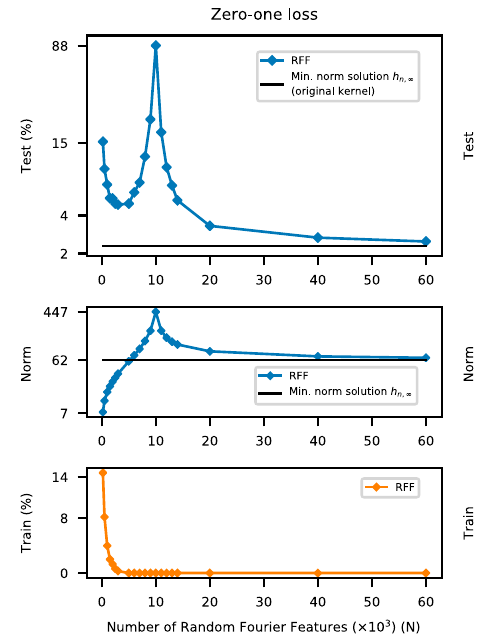
\includegraphics[height=7cm]{RFF-results.png}
\end{frame}

\begin{frame}
\frametitle{Empirical Evidence - Neural Networks}
Neural Networks. (Might be hard to explain why SGD is the inductive bias.)
\end{frame}


\begin{frame}
\frametitle{Appendix on Approximation Theorem}
On why they choose a function with a smaller norm in RKHS.
\end{frame}

\end{document} 
